\documentclass[8pt,landscape,letterpaper]{extarticle}
\usepackage[utf8]{inputenc}
\usepackage[ngerman]{babel}
\usepackage[T1]{fontenc}
\usepackage{mathtools}
%\usepackage[LY1,T1]{fontenc}
%\usepackage{frutigernext}
%\usepackage[lf,minionint]{MinionPro}
\usepackage{tikz}
\usetikzlibrary{shapes,positioning,arrows,fit,calc,graphs,graphs.standard}
\usepackage[nosf]{kpfonts}
\usepackage[t1]{sourcesanspro}
\usepackage{multicol}
\usepackage{wrapfig}
\usepackage[top=0mm,bottom=1mm,left=0mm,right=1mm]{geometry}
\usepackage[framemethod=tikz]{mdframed}
\usepackage{microtype}
\usepackage{pdfpages}
\usepackage{bbm}
\usepackage{listings}
\usepackage{color}
\usepackage{spverbatim}
\usepackage{lipsum}
\usepackage{graphicx}
\graphicspath{ {./images/} }


\let\bar\overline

\definecolor{myblue}{cmyk}{1,.72,0,.38}

\def\firstcircle{(0,0) circle (1.5cm)}
\def\secondcircle{(0:2cm) circle (1.5cm)}

\colorlet{circle edge}{myblue}
\colorlet{circle area}{myblue!5}

\tikzset{filled/.style={fill=circle area, draw=circle edge, thick},
    outline/.style={draw=circle edge, thick}}
    
\pgfdeclarelayer{background}
\pgfsetlayers{background,main}

\everymath\expandafter{\the\everymath \color{myblue}}
\everydisplay\expandafter{\the\everydisplay \color{myblue}}

\renewcommand{\baselinestretch}{.8}
\pagestyle{empty}

\global\mdfdefinestyle{header}{%
linecolor=gray,linewidth=1pt,%
leftmargin=0mm,rightmargin=0mm,skipbelow=0mm,skipabove=0mm,
}

\newcommand{\header}{
\begin{mdframed}[style=header]
\footnotesize
\sffamily
~Page~\thepage~of~4
\end{mdframed}
}

\makeatletter 
% based on: https://tex.stackexchange.com/questions/218587/how-to-set-one-header-for-each-page-using-multicols
\renewcommand{\section}{\@startsection{section}{1}{0mm}%
                                {.2ex}%
                                {.2ex}%x
                                {\color{myblue}\sffamily\small\bfseries}}
\renewcommand{\subsection}{\@startsection{subsection}{1}{0mm}%
                                {.2ex}%
                                {.2ex}%x
                                {\sffamily\bfseries}}

\newenvironment{simplebsl}{%
   \catcode`\#=12
   \catcode`\^=12
   \catcode`\_=12
   \catcode`\~=12
   \catcode`\%=12
   \catcode`\(=12
   \catcode`\)=12
   \catcode`\[=12
   \catcode`\]=12
}{}



\makeatother
\setlength{\parindent}{0pt}

\begin{document}
%\footnotesize
\small
\begin{multicols*}{6}

\section{Gathering and Collecting Data}
\subsection*{Tools}
https://toolbox.google.com/datasetsearch
\subsection*{Human Subjects in Research}
Why? $\rightarrowtail$ Tuskegee Syphilis trials. \\
Reaction: 
\begin{enumerate}
    \item HHS Regulations for the Protection of Human Subjects at Title 45 Code of Federal Regulations Part 46. 
    \item Belmont report (designed for biomedical research). 
\end{enumerate}
\textbf{Principles of Belmont report: }
\begin{enumerate}
   \item Respect for Persons
   \begin{itemize}
     \item Informed consent (subjects must be known aboout the purpose of the experiment)
     \item Protecting privacy and maintaining confidentiality
     \item Additional safeguards for protection of subjects likely to be vulnerable to coercion or undue influence
   \end{itemize}
   \item Beneficence
   \begin{itemize}
     \item Assessment of risk/benefit analysis including study design
     \item Ensure that risks to subjects are minimized
     \item Risk justified by benefits of the research
   \end{itemize}
   \item Justice
   \begin{itemize}
     \item Ensure that selection of subjects is equitable
   \end{itemize}
\end{enumerate}
\textit{Code: }
\begin{spverbatim}
# library(tibble)
# library(tidyverse)
successes <- rbinom(1000,8,0.2)
data <- as_tibble(data.frame(successes))

bin_data <- data %>% group_by(successes) %>% 
  summarise(n=n()) %>% 
  mutate(freq=n/sum(n))
  
cdf_data <- data %>% group_by(successes) %>% 
  summarise(n=n()) %>% arrange(desc(successes)) %>% 
  mutate(freq=n/cumsum(n))
\end{spverbatim}

\section{Bayes Theorem}
\subsection*{Temporal Inferrence}
Given $\mathbf{G}$: \\
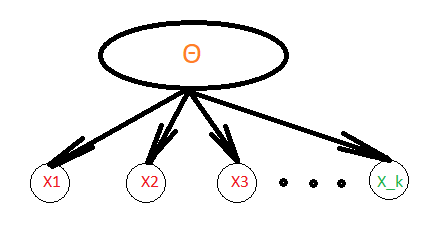
\includegraphics[width=\columnwidth]{bayes}
As $d\_sep_{\mathbf{G}}(X_{i},X_{j}|\theta)$,\\

$\mathbf{P}(x_k|x_1,x_2,\ldots,x_{k-1}) = \sum_{\theta}{\mathbf{P}(x_k|\theta)\mathbf{P}(\theta|x_1,x_2,\ldots,x_{k-1})}$\\

\textit{Code: }
\begin{spverbatim}
# theta = 0.001 # the initial condition
p_x = 0.99
p_n_x = 0.05

# X_1 is +
theta = p_x*theta/(p_x*theta+p_n_x*(1-theta))
theta
\end{spverbatim}

\section{Experimental Design}
\subsection*{Power Calculations in Practice}
$\Phi^{-1}(1-\beta)+\frac{\tau}{\sigma'}=\Phi^{-1}(1-\frac{\alpha}{2})$\\
Therefore,
$N=\frac{(\Phi^{-1}(\beta)+\Phi^{-1}(1-\frac{\alpha}{2}))^2}{\frac{\tau^2}{\sigma^2}\gamma(1-\gamma)}$\\
\textit{Code: }
\begin{spverbatim}
# Two-sided test
power=0.95
level=0.05
tau=0.5
lambda=0.5 # the sample-bias ratio N_t/N
sigma=2
N = (qnorm(power) + qnorm(1 - level/2))^2/((tau / sigma)^2*lambda*(1 - lambda))
# or (when tau is large)
pwr_values = pwr.2p.test(h=tau/sigma, sig.level=level, power=power)
N = pwr_values$n*2
\end{spverbatim}

\subsection*{Wald Test}
(See \textit{\textbf{Two Stage Least Squares}} section)\\
\textit{\textbf{Note: }Even a "tiny" violation of either of the conditions for the validity of the instrument can result in very large bias. Any bias in the reduced form will be "blown up" when it's divided by the first stage difference. }

\subsection*{Regression Discontinuity Design}
\textbf{\textit{Assumption: }}This test will be informative when manipulation of the running variable is monotonic. \\
\textit{Code: }
\begin{spverbatim}
install.packages("rdd")
library(rdd)
indiv <- read.csv('indiv_final.csv')
indiv$above <- as.numeric(indiv$difshare > 0)

dc = DCdensity(indiv$difshare, 0, ext.out=TRUE)
abline(v=0)
# The difference in the log estimate in heights at the cutpoint
dc$theta

#Parametric Regression
matrix_coef <- matrix(NA, nrow = 2, ncol = 11)

model <- lm(myoutcomenext ~ above, data = indiv, subset = abs(difshare) <= 0.5)
matrix_coef[1, 1] <- model$coefficients[2]
pvalue <- summary(model)
matrix_coef[2, 1] <- pvalue$coefficients[2, 4]

#Non-parametric Regression
model <- RDestimate(myoutcomenext~difshare, data=indiv, subset = abs(indiv$difshare) <=0.5)
summary(model)
plot(model)
\end{spverbatim}

\subsection*{Two Stage Least Squares}
\textbf{Endogeneity: }In econometrics, endogeneity broadly refers to situations in which an explanatory variable is correlated with the error term. 
\begin{itemize}
    \item \textit{Expression: }Unable to control an explanatory variable properly. 
    \item \textit{Reasons: }Endogeneity can be OVB, reverse causality and measurement error. 
\end{itemize}
\textbf{Assumption: }Exclusion Restriction. \\
\textbf{Note: }Must have at least as many instruments as you have endogenous explanatory variables (this is referred to as the "rank condition"). \\
\textit{Code: }
\begin{spverbatim}
iva1 <- ivreg(workedm ~ three + blackm + hispm + othracem |
                blackm + hispm + othracem + multiple, data = census80)
IVa[1, 1] <- iva$coefficients[2]
pvalue <- summary(iva1)
IVa[2, 1] <- pvalue$coefficients[2, 4]
\end{spverbatim}

\subsection*{Phase-in Design}
\begin{itemize}
    \item Choose target individuals or communities to be covered over several years
    \item Randomize the order in which they are phased in
    \item Those not yet phased in are the comparison
\end{itemize}


\section{Regression Analysis in Practice}
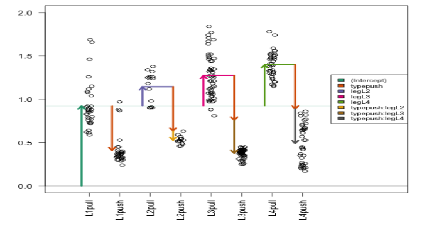
\includegraphics[width=\columnwidth]{did}

\subsection*{Categorical Variables}
\textbf{Treatment and Control Group: } \\
$Y_i=\alpha+\beta D_i + \gamma X_i + \epsilon_i$\\
In this case $\beta$ is the difference in intercept between group \textbf{\textit{A}} and group \textbf{\textit{B}}. This is the most frequent way that RCT are analyzed: the matrix X are "control" variables. 

\subsection*{Difference-in-Difference}
\textbf{\{Treatment, Control\}$\times$\{Male, Female\}: } \\
$Y_i=\alpha+\beta D_i + \gamma M_i + \delta M_i \ast D_i + \epsilon_i$ \\
So, $\delta$ is the difference between group \textbf{\textit{Male}} and group \textbf{\textit{Female}} in difference between group \textbf{\textit{Treatment}} and group \textbf{\textit{Control}}. \\
\textit{\textbf{Assumption: }Parallel trends assumption. }\\
\textit{\textbf{Causal interpretation: }If you cannot credibly claim that the parallel trends assumption is satisfied, then estimates obtained from a differences-in-differences design cannot be interpreted causally. }

\subsection*{Local Linear Regression}
\begin{itemize}
    \item Define the dummies as: \\
    $D_{1i} = I_{X_0 \leq X_{1i} < X_1}$\\
    $D_{2i} = I_{X_1 \leq X_{1i} < X_2}$
    \item Run regression: \\
    $Y_i=\beta_1 D_{1i} + \beta_2 D_{2i} + \dots + \beta_J D_{Ji} + \epsilon_i$
    \item Define Piece wise linear variables. 
\end{itemize}

\subsection*{Omitted Variable Bias}
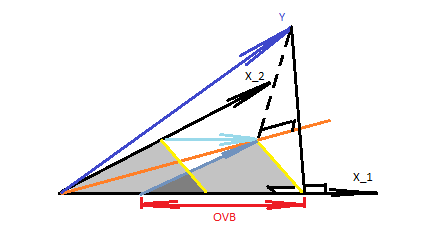
\includegraphics[width=\columnwidth]{ovb}
Correct model: $Y_i=\beta_0+\beta_1 X_{1i}+\beta_2 X_{2i}+\epsilon_i$\\
Estimated model: $Y_i=\alpha_0+\alpha_1 X_{1i}+w_i$\\
Define Ancillary (or Auxillary) regression: $X_{2i}=\delta_0+\delta_1 X_{1i}+\zeta_i$\\
Then,\\
${OVB}=\hat{\alpha_1}-\beta_1=\delta_1 \beta_2$


\section{Describling Data}
\textit{Code: }
\begin{spverbatim}
#Preliminaries
rm(list=ls())
library("tidyverse")

setwd("E:/")

#Getting the data
gender_data <- as_tibble( read.csv( "Gender_StatsData.csv" ) )
head(gender_data)

teenager_fr <- gender_data %>% filter(Indicator.Code == "SP.ADO.TFRT")
byincomelevel <- filter(teenager_fr, Country.Code%in%c("LIC","MIC") | Country.Code%in%c("HIC"))
plotdata_bygroupyear <- gather(byincomelevel, Year, FertilityRate, X1960:X2015) %>% 
  select(Year, ï..Country.Name, Country.Code, FertilityRate)
plotdata_byyear <- plotdata_bygroupyear
# drops = "Country.Name"
# plotdata_byyear = dummy.data.frame(plotdata_byyear, "Country.Name", sep=".")
# plotdata_byyear = plotdata_byyear[, !(colnames(plotdata_byyear) %in% drops)]
plotdata_byyear <- plotdata_byyear %>% select(Year, Country.Code, FertilityRate) %>% 
  spread(Country.Code, FertilityRate)

rm(gender_data)

every_nth = function(n) {
  return(function(x) {x[c(TRUE, rep(FALSE, n - 1))]})
}
p = ggplot(plotdata_bygroupyear, aes(x=Year, y=FertilityRate, group=Country.Code, col=Country.Code))
p = p + scale_x_discrete(breaks = every_nth(n=5))
p = p + theme(axis.text.x = element_text(angle = 90))
p = p + geom_line()
p
\end{spverbatim}

\section{Basic Simulation}
If $F(y)$ is a monotic function and $X \sim \mathcal{U}[0, 1]$ then,\\
$Y = F^{-1}(X)$ has PDF is $F(y)$
\section{Basic Visualization}
\textit{Code: }
\begin{spverbatim}
#scatter, regression, and sample mean plot
p <- ggplot()
p <- p+geom_point(data=demo, aes(x=FHouse, y=GDP), color="purple")
p <- p+geom_smooth(data=demo, method="lm", aes(x=FHouse, y=GDP))
p <- p+geom_point(data=meanGDP, aes(x=FHouse,y=GDPmean), color="orange")
p

# or
# ggplot(dat, aes(x=head_edu )) + geom_density(data=subset(dat, treat_invite==0), fill = "red", alpha=0.2) + geom_density(data=subset(dat, treat_invite==1), fill = "blue", alpha=0.2)
# ggplot(dat, aes(x=mosques )) + geom_density(data=subset(dat, treat_invite==0), fill = "red", alpha=0.2) + geom_density(data=subset(dat, treat_invite==1), fill = "blue", alpha=0.2)
# ggplot(dat, aes(x=pct_poor )) + geom_density(data=subset(dat, treat_invite==0), fill = "red", alpha=0.2) + geom_density(data=subset(dat, treat_invite==1), fill = "blue", alpha=0.2)
# ggplot(dat, aes(x=total_budget )) + geom_density(data=subset(dat, treat_invite==0), fill = "red", alpha=0.2) + geom_density(data=subset(dat, treat_invite==1), fill = "blue", alpha=0.2)
\end{spverbatim}
\section{Basic Regression}
\textit{Code: }
\begin{spverbatim}
#simple linear regression
single <- lm(lwage ~ yrs_school, data = nlsw88)
summary(single) # show results
coefficients(single) # model coefficients
ci <- confint(single, level=0.9) 
ci
resid <- residuals(single) # residuals
sum(resid)
\end{spverbatim}

\section{Causality and Non-parametric Regression}
\subsection*{Rubin Causal Model}
For any unit, the causal effect of a treatment is the difference between the potential outcome with and without the treatment. \\
$\rightarrowtail$ Need to define treatment effects for each possibility. \\
Because that at most one of the potential outcomes can be observed, some assumptions are neccesary: 
\subsection*{SUTVA (Stable Unit Treatment Value Assumption)}
\textbf{\textit{Assumption: }}The potential outcome for any unit do not vary with the treatments assigned to other units and, for each unit, there are no different forms or versions of each treatment unit leading to different outcomes. 
\subsection*{Kernel Regression}
\textbf{\textit{Formula: }} \\
$\hat{f}_h(x) = \frac{1}{n} \sum_{i=1}^{n} K_h(x-x_i) = \frac{1}{nh}\sum_{i=1}^{n} K(\frac{x-x_i}{h})$ \\
\textit{Code: }
\begin{spverbatim}
#Preliminaries
rm(list=ls())
library(perm) # chooseMatrix()
library(np)
setwd("E:/")
schools <- read.csv("teachers_final.csv")
attach(schools)
bw_a <-npreg(xdat=pctpostwritten, ydat= open, bws=0.04,bandwidth.compute=FALSE)
plot(bw_a)


treat <- schools$pctpostwritten[treatment==1]
cont <- schools$pctpostwritten[treatment==0]

ks.test(treat, cont, "greater")

schools$group[schools$treatment==1] <-"T"
schools$group[schools$treatment==0] <-"C"
ggplot(schools, aes(pctpostwritten,colour = group)) + stat_ecdf()
\end{spverbatim}

\section{Confidence Intervals}

Let $\displaystyle ( E,(\mathbb{P}_{\theta })_{\theta \in \Theta })$ be a statistical  model based on observations $X_{1} , \ldots X_{n}$  and assume $\displaystyle \Theta \subseteq \mathbb{R}$. Let $\displaystyle \alpha \in ( 0,1)$.\\

\textbf{Non asymptotic} confidence interval of level $\displaystyle 1-\alpha $ for $\displaystyle \theta $:\\

Any random interval $\displaystyle \mathcal{I}$, depending on the sample $X_{1} , \ldots X_{n}$ but not at $\displaystyle \theta $ and such that:\\

$\mathbb{P}_{\theta }[\mathcal{I} \ni \theta ] \geq 1-\alpha ,\ \ \forall \theta \in \Theta$\\

Confidence interval of \textbf{asymptotic level} $\displaystyle 1-\alpha $  for $\displaystyle \theta $:\\

Any random interval $\displaystyle \mathcal{I}$ whose boundaries do not depend on $\displaystyle \theta $ and such that:\\

$\lim _{n\rightarrow \infty }\mathbb{P}_{\theta } [\mathcal{I} \ni \theta ]\geq 1-\alpha ,\ \ \forall \theta \in \Theta $\\

\subsection*{Two-sided asymptotic CI}
Let $X_1, \ldots, X_n = \tilde{X}$ and $\tilde{X}\stackrel{iid} {\sim} P_{\theta}$. A two-sided CI is a function depending on $\tilde{X}$ giving an upper and lower bound in which the estimated parameter lies $\mathcal{I} = [l(\tilde{X},u(\tilde{X})]$ with a certain probability $\mathbb{P}(\theta \in  \mathcal{I}) \geq 1 -q_{\alpha}$ and conversely $\mathbb{P}(\theta \not\in  \mathcal{I}) \leq \alpha$\\

Since the estimator is a r.v. depending on $\tilde{X}$ it has a variance $Var(\hat{\theta}_n$ and a mean $\mathbb{E}[\hat{\theta}_n]$. After finding those it is possible to standardize the estimator using the CLT. This yields an asymptotic CI: $\mathcal{I} = \hat{\theta}_n + [\frac{-q_{\alpha /2} \sqrt{Var(\theta)} }{\sqrt{n}}, \frac{q_{\alpha /2} \sqrt{Var(\theta)} }{\sqrt{n}}]$

This expression depends on the real variance $Var(\theta)$ of the r.vs, the variance has to be estimated. Three possible methods: plugin (use sample mean), solve (solve quadratic inequality), conservative (use the maximum of the variance).\\

\subsection*{Delta Method}

If I take a function of the mean and want to make it converge to a function of the mean. 

$\sqrt{n}(g(\widehat{m}_1) - g(m_1(\theta ))) \xrightarrow [n \to \infty ]{(d)} \mathcal{N}(0, g'(m_1(\theta ))^2 \sigma ^2)$


\section{Hypothesis Testing}
\subsection*{Comparisons of two proportions}

Let $X_1,\dots ,X_ n \stackrel{iid}{\sim} Bern(p_x)$ and  $Y_1,\dots ,Y_ n \stackrel{iid}{\sim} Bern(p_y)$ and be $X$ independent of $Y$. $\hat{p}_x= 1/n \sum_{i=1}^{n} X_i$ and $\hat{p}_x= 1/n \sum_{i=1}^{n} Y_i$\\

$H_0: p_x = p_y; H_1: p_x \neq p_y$

To get the asymptotic Variance use multivariate Delta-method. Consider $\hat{p}_x - \hat{p}_y = g(\hat{p}_x,\hat{p}_y); g(x,y)= x -y$, then

$\sqrt(n) (g(\hat{p}_x,\hat{p}_y) - g(p_x-p_y)) \xrightarrow[n \rightarrow \infty]{(d)} N(0,\nabla g(p_x-p_y)^T \Sigma \nabla g(p_x-p_y))$\\ 

$\Rightarrow N(0,p_x(1-px) + p_y(1-py))$

Pivot:\\

Let $X_1,\dots ,X_ n$ be random samples and let $T_ n$  be a function of $X$ and a parameter vector $\theta$. That is, $T_n$ is a function of $X_1,\dots ,X_ n,\theta$. Let $g(T_ n)$ be a random variable whose distribution is the same for all $\theta$ . Then, $g$ is called a pivotal quantity or a pivot.\\

For example, let $X$ be a random variable with mean $\mu$ and variance $\sigma^2$ . Let $X_1,\dots ,X_ n$ be iid samples of $X$. Then,

$$\displaystyle  g_ n \triangleq \frac{\overline{X_ n} - \mu }{\sigma }$$
 		 	 
is a pivot with $\theta = \left[\mu ~ ~  \sigma ^2\right]^ T$ being the parameter vector. The notion of a parameter vector here is not to be confused with the set of paramaters that we use to define a statistical model. 			 
\subsection{KS Test}
\textit{Code: }
\begin{spverbatim}
x=sort(c(.28,.2,.01,.8,.1))
n=length(x)
mu=mean(x)
sigma=sd(x)
y=pnorm((x - mu)/sigma)
ids1=seq(1,n,1)/n
ids2=rep(0,n)
ids2[-1]=ids1[-n]
T_n = max(cbind(abs(y - ids1),abs(y - ids2)))*sqrt(n)
T_table = T_n/sqrt(n)
T_table
\end{spverbatim}

\subsection{Walds Test and Log Test}
$\, X_1, \ldots , X_ n \stackrel{iid}{\sim } \mathbf{P}_{\theta ^*}$  for some true parameter $\theta ^* \in \mathbb {R}^ d$. We construct the associated statistical model $(\mathbb {R}, \{  \mathbf{P}_\theta \} _{\theta \in \mathbb {R}^ d } )$ and the maximum likelihood estimator $\widehat{\theta }_ n^{MLE}$ for $\theta ^*$.

Decide between two hypotheses:

$H_0: \displaystyle  \theta ^* = \mathbf{0}$ VS $H_1: \displaystyle  \theta ^* \neq \mathbf{0}$

Assuming that the null hypothesis is true, the asymptotic normality of the MLE $\widehat{\theta }_ n^{MLE}\,$ implies that the following random variable $\left\lVert \sqrt{n}\, \mathcal{I}(\mathbf{0})^{1/2}(\widehat{\theta }_ n^{MLE}- \mathbf{0}) \right\rVert ^2$ converges to a $\chi ^2_ k$ distribution.\\

$\left\lVert \sqrt{n}\, \mathcal{I}(\mathbf{0})^{1/2}(\widehat{\theta }_ n^{MLE}- \mathbf{0}) \right\rVert ^2 \xrightarrow [n\to \infty ]{(d)} \chi ^2_ d\,$\\

Wald's Test in 1 dimension:\\

In 1 dimension, Wald's Test coincides with the two-sided test based on on the asymptotic normality of the MLE.

Given the hypotheses

$H_0: \displaystyle  \theta ^* = \mathbf{0}$ VS $H_1: \displaystyle  \theta ^* \neq \mathbf{0}$	 	 
 	 		 	 
a two-sided test of level $\alpha$, based on the asymptotic normality of the MLE, is $\displaystyle  \displaystyle \psi _\alpha =\mathbf{1}\left(\sqrt{nI(\theta _0)} \left| \widehat{\theta }^{\text {MLE}} -\theta _0 \right|>q_{\alpha /2}(\mathcal{N}(0,1))\right)$

 		 	 
where the Fisher information $\, I(\theta _0)^{-1}\,$ is the asymptotic variance of $\, \widehat{\theta }^{\text {MLE}}\,$ under the null hypothesis.

On the other hand, a Wald's test of level $\alpha$ is

$\displaystyle  \displaystyle \psi ^{\text {Wald}}_\alpha	= \displaystyle \mathbf{1}\left(nI(\theta _0) \left(\widehat{\theta }^{\text {MLE}} -\theta _0\right)^2\, >\, q_{\alpha }(\chi ^2_1)\right) = \displaystyle \mathbf{1}\left(\sqrt{nI(\theta _0)} \, \left| \widehat{\theta }^{\text {MLE}} -\theta _0 \right|\, >\, \sqrt{q_{\alpha }(\chi ^2_1)}\right).$			 	 
 
\textit{Code: }
\begin{spverbatim}
# pdf: lambda*e^(-lambda)
# H0: lambda = 1; H1: otherwise
# MLE estimate: 100/120 = n/Sigma
# Wald test
1 - pchisq(100*((100/120 - 1)^2)/((100/120)^2),df=1)
# Log test. 
# This test is less conservative than the Wald test
1 - pchisq(((100*log(100/120)+(-(100/120)*120)) - (100*log(1)+(-(1)*120)))*2,df=1)
\end{spverbatim}

\subsection{Welch T-test}
\textit{Code: }
\begin{spverbatim}
samplesA = c(1,3)
samplesB = c(3,3,2)
n=length(samplesA)
m=length(samplesB)
meanA = mean(samplesA)
meanB = mean(samplesB)
varA = var(samplesA)
varB = var(samplesB)
N = (varA/n + varB/m)^2/(varA^2/n^2/(n - 1)+varB^2/m^2/(m - 1))
T_N = (meanA - meanB)/sqrt(varA/n + varB/m)
p_value = 1 - pt(T_N, df=N)
p_value
\end{spverbatim}

\subsection{ANOVA}
\textit{Memic: } If $X \sim \chi_n^2$ and $Z \sim \chi_m^2$ and they're independent, then\\
$\frac{X/n}{Z/m} \sim F_{n,m}$\\
\textit{Code: }
\begin{spverbatim}
library(car)
model <- lm(GDP ~ FHouse_sq + FHouse, demo)
summary(model)
anova_rest <- anova(model)

#Test
statistic_test <- (((anova_rest$`Sum Sq`[2]-anova_unrest$`Sum Sq`[3])/(anova_unrest$Df[2]))
                   /((anova_unrest$`Sum Sq`[3])/anova_unrest$Df[3]))
statistic_test
pvalue <- df(statistic_test, 1, anova_unrest$Df[3])
pvalue

matrixR <- c(0, -1, 1)
linearHypothesis(model, matrixR)

# or 
# fitTL <- lm(friction ~ type + leg, data=spider)
# library(contrast) #Available from CRAN
# L3vsL2 <- contrast(fitTL, list(leg="L3", type="pull"), list(leg="L2", type="pull"))
# L3vsL2
\end{spverbatim}

\section{Random Vectors}


A random vector $\mathbf X= \left(X^{(1)},\dots ,X^{(d)}\right)^ T$ of dimension $d \times 1$ is a vector-valued function from a probability space $\omega$ to $\mathbb {R}^ d$:\\

$  \mathbf{X}\, \, :\,  \Omega \longrightarrow   \mathbb {R}^ d$\\

$ \omega  \longrightarrow  \begin{pmatrix}  X^{(1)}(\omega ) \\ X^{(2)}(\omega )\\ \vdots \\ X^{(d)}(\omega )\end{pmatrix}$\\

where each $\, X^{(k)}\ $, is a (scalar) random variable on $\Omega$. \\

PDF of $\mathbf X$: joint distribution of its components $X^{(1)},\, \ldots ,\, X^{(d)}$. \\

CDF of $\mathbf X$:\\

$\mathbb {R}^ d \rightarrow   [0,1]$\\

$ \mathbf{x}  \mapsto   \mathbf{P}(X^{(1)}\leq x^{(1)},\ldots ,\, X^{(d)}\leq x^{(d)}).$\\

The sequence $\mathbf{X}_1, \mathbf{X}_2,\ldots$ converges in probability to $\mathbf{X}$ if and only if each component of the sequence $\, X_1^{(k)},X_2^{(k)},\ldots \,$ converges in probability to $\, X^{(k)}$.


\subsection*{Expectation of a random vector}
The expectation of a random vector is the elementwise expectation. Let $\mathbf X$  be a random vector of dimension $d \times 1$.\\

$   \mathbb E[\mathbf X] =  \begin{pmatrix} \mathbb E[X^{(1)}]\\ \vdots \\ \mathbb E[X^{(d)}]\end{pmatrix}.$\\

The expectation of a random matrix is the expected value of each of its elements. Let $X=\{X_{ij}\}$ be an $n \times p$ random matrix. Then $\mathbb{E}[X]$, is the $n \times p$ matrix of numbers (if they exist):\\

$\mathbb{E}[X]= \begin{bmatrix}
   \mathbb{E}[X_{11}]       & \mathbb{E}[X_{12}] & \dots & \mathbb{E}[X_{1p}] \\
   \mathbb{E}[X_{21}]       & \mathbb{E}[X_{22}] & \dots & \mathbb{E}[X_{2p}] \\
    \vdots & \vdots &\ddots & \vdots \\
     \mathbb{E}[X_{n1}]       & \mathbb{E}[X_{n2}] & \dots & \mathbb{E}[X_{np}] \\
\end{bmatrix}$\\

Let $X$ and $Y$ be random matrices of the same dimension, and let $A$ and $B$ be conformable matrices of constants.\\

$\mathbb{E}[X + Y] = \mathbb{E}[X] + \mathbb{E}[Y]$\\
$\mathbb{E}[AXB] = A \mathbb{E}[X] B$\\


\subsection*{Covariance Matrix}
Let $X$  be a random vector of dimension $d \times 1$ with expectation $\mu _{X}$. 

Matrix outer products!\\ 

$\Sigma =\mathbb E[(X- \mu _{X})(X- \mu _{X})^ T] =$\\

$\mathbb{E}  \begin{pmatrix} \begin{bmatrix} 

X_1 - \mu_1\\
X_2 - \mu_2\\
\ldots\\
X_d - \mu_d\\

\end{bmatrix} \begin{bmatrix} X_1 - \mu_1, X_2 - \mu_2,\ldots, X_d - \mu_d \end{bmatrix} \end{pmatrix}$\\

$\Sigma = Cov (X) = \begin{bmatrix}
\sigma_{11} & \sigma_{12} &\ldots & \sigma_{1d} \\
\sigma_{21} & \sigma_{22} &\ldots & \sigma_{2d} \\
\vdots & \vdots &\ddots & \vdots \\
\sigma_{d1} & \sigma_{d2} &\ldots & \sigma_{dd} \\

\end{bmatrix}$\\

The covariance matrix $\Sigma$ is a $d \times d$ matrix. It is a table of the pairwise covariances of the elemtents of the random vector. Its diagonal elements are the variances of the elements of the random vector, the off-diagonal elements are its covariances. Note that the covariance is commutative e.g. $\sigma_{12} = \sigma_{21}$ \\

Alternative forms:\\

$\Sigma = \mathbb {E}[XX^ T] - \mathbb {E}[X]\mathbb {E}[X]^ T =\\ = \mathbb {E}[XX^ T] - \mu _{X}\mu _{X}^ T$\\

Let the random vector $X \in \mathbb{R}^d$ and $A$ and $B$ be conformable matrices of constants.\\

$Cov(AX + B) = Cov(AX) = A Cov(X) A^T = A \Sigma A^T$

Every Covariance matrix is positive definite.\\

$\Sigma \prec 0$\\

\subsection*{Gaussian Random Vectors}


A random vector $\mathbf{X}=(X^{(1)},\ldots ,X^{(d)})^ T\,$ is a Gaussian vector, or multivariate Gaussian or normal variable, if any linear combination of its components is a (univariate) Gaussian variable or a constant (a “Gaussian" variable with zero variance), i.e., if $\alpha ^ T \mathbf{X}$ is (univariate) Gaussian or constant for any constant non-zero vector $\alpha \in \mathbb {R}^ d$.

\subsection*{Multivariate Gaussians}

The distribution of, $X$ the $d$-dimensional Gaussian or normal distribution, is completely specified by the vector mean $\mu =\mathbb E[\mathbf{X}]= (\mathbb E[X^{(1)}],\ldots ,\mathbb E[X^{(d)}])^ T$ and the $d \times d$ covariance matrix $\Sigma$. If $\Sigma$ is invertible, then the pdf of $X$ is:\\

$   f_{\mathbf X}(\mathbf x) = \frac{1}{\sqrt{\left(2\pi \right)^ d \text {det}(\Sigma )}}e^{-\frac{1}{2}(\mathbf x-\mu )^ T \Sigma ^{-1} (\mathbf x-\mu )}, ~ ~ ~ \\ \mathbf x\in \mathbb {R}^ d$\\


Where $\text {det}(\Sigma )$ is the determinant of $\Sigma$, which is positive when $\Sigma$ is invertible.

If $\mu = 0$ and $\Sigma$ is the identity matrix, then $X$ is called a standard normal random vector .

If the covariant matrix $\Sigma$ is diagonal, the pdf factors into pdfs of univariate Gaussians, and hence the components are independent.\\

The linear transform of a gaussian $X \thicksim N_d(\mu,\Sigma)$ with conformable matrices $A$ and $B$ is a gaussian:\\ 

$AX + B = N_d(A\mu + b, A \Sigma A^T)$

\subsection*{Multivariate CLT}

Let $X_1, \ldots, X_d \in \mathbb{R}^d$ be independent copies of a random vector $X$
such that $\mathbb{E}[x] = \mu$ ($d \times 1$ vector of expectations) and $Cov(X)= \Sigma$\\

$\sqrt(n)(\bar{X_n}-\mu) \xrightarrow[n \rightarrow \infty]{(d)} N(0,\Sigma)$\\

$\sqrt(n) \Sigma^{-1/2} \bar{X_n}-\mu \xrightarrow[n \rightarrow \infty]{(d)} N(0,I_d)$\\

Where $\Sigma^{-1/2}$ is the $d \times d$ matrix such that $\Sigma^{-1/2} \Sigma^{-1/2} = \Sigma^{1}$ and $I_d$ is the identity matrix.\\

\subsection*{Multivariate Delta Method}

Gradient Matrix of a Vector Function:\\

Given a vector-valued function $f:\mathbb {R}^ d \to \mathbb {R}^ k$, the gradient or the gradient matrix of $f$, denoted by $\nabla f$ , is the $d \times k$ matrix:\\

$   \nabla f =\\ = \begin{pmatrix} |& |& |& |\\ \nabla f_1&  \nabla f_2& \ldots & \nabla f_ k\\ |& |& |& |\\ \end{pmatrix} = \\
= \begin{pmatrix} \frac{\partial f_1}{\partial x_1}& \ldots & \frac{\partial f_ k}{\partial x_1}\\ \vdots & \ldots & \vdots \\ \frac{\partial f_1}{\partial x_ d}& \ldots & \frac{\partial f_ k}{\partial x_ d} \end{pmatrix}.$\\

This is also the transpose of what is known as the Jacobian matrix $\mathbf{J}_ f$ of $f$.\\

General statement, given\\

\begin{itemize}
	\item $\left(\mathbf{T}_ n\right)_{n\geq 1}$ a sequence of random vectors 
	\item satisfying $\,  \sqrt{n} \left(\mathbf{T}_ n - \vec{\theta } \right) \xrightarrow [n\to \infty ]{(d)} \mathbf{T}$,

	\item a function $\mathbf{g}:\mathbb {R}^ d\to \mathbb {R}^ k$  that is continuously differentiable at $\vec{\theta }$,

\end{itemize}

then\\

$   \sqrt{n} \left(\mathbf{g}(\mathbf{T}_ n) - \mathbf{g}(\vec{\theta }) \right) \xrightarrow [n\to \infty ]{(d)} \nabla \mathbf{g}(\vec{\theta })^ T\, \mathbf{T}\qquad$\\

With multivariate Gaussians and Sample mean:\\

Let $\mathbf{T}_ n=\overline{\mathbf{X}}_ n$ where $\overline{\mathbf{X}}_ n$ is the sample average of $\, \mathbf{X}_1,\ldots ,\mathbf{X}_ n\, \stackrel{iid}{\sim }\mathbf{X},\,$ and $\, \vec{\theta }=\mathbb E[\mathbf{X}].\, \,$ The (multivariate) CLT then gives $\, \mathbf{T}\sim \mathcal{N}(\mathbf{0},\Sigma _\mathbf{X})$ where $\, \Sigma _\mathbf{X}\,$ is the covariance of $\mathbf{X}.\, \,$ In this case, we have:\\

$\sqrt{n} \left(\mathbf{g}(\mathbf{T}_ n) - \mathbf{g}(\vec{\theta }) \right) \xrightarrow [n\to \infty ]{(d)} \nabla \mathbf{g}(\vec{\theta })^ T\mathbf{T}\,$\\

$\nabla \mathbf{g}(\vec{\theta })^ T\mathbf{T} \sim \,  \mathcal{N}\left(0, \nabla \mathbf{g}(\vec{\theta })^ T \Sigma _{\mathbf{X}} \nabla \mathbf{g}(\vec{\theta })\right)\qquad$\\

$(\mathbf{T}\sim \mathcal{N}(\mathbf{0},\Sigma _\mathbf{X}))$\\

\section{Generalized Linear Models}
We relax the assumption that $\mu$ is linear. Instead, we assume that g $\circ \mu$ is linear, for some function $g$:\\

$g(\mu (\mathbf x)) = \mathbf x^ T \beta$

The function $g$ is assumed to be known, and is referred to as the link function. It maps the domain of the dependent variable to the entire real Line.

it has to be strictly increasing,

it has to be continuously differentiable and

its range is all of $\mathbb{R}$

\subsection{Multivariate Linear Regression}
\textbf{\textit{[R]}}
\begin{simplebsl}
\\Setup: Y = X%*%Beta + e
\\Modeling Assumptions in Linear Regression:
\\1. Linear Relationship. 
\\2. X ~ Normal, e_i ~(idd) Normal(mu=0, sigma^2)
\\3. E[e_i*e_j] = 0, E[X*e_j] = 0
\\Beta_hat ~ Normal(Beta, sigma^2*solve(trans(X)%*%X))
\\sigma_hat^2 = trans(Y - X%*%Beta_hat)%*%(Y - X%*%Beta_hat)/(n - p)
\end{simplebsl}

\subsection{Theorems for Hypothesis Testing:}
\textbf{\textit{[R]}}
\begin{simplebsl}
\\1. n*pop_var/sigma^2 ~ Chi-square(n - p)
\\2. Cochran's theorem. 
\end{simplebsl}

\subsection{T Test:}
\textbf{\textit{[R]}}
\begin{simplebsl}
\\T_n = trans(u)
\\%*%(Beta_hat - Beta)
\\/sigma_hat
\\*sqrt(trans(u)%*%solve(trans(X)%*%X)%*%u)
\\T_n ~ T(n-p)
\end{simplebsl}

\subsection{Canonical Exponential Family:}
\textbf{\textit{[R]}}
\begin{simplebsl}
\\f_theta(y) = e^((y*theta-b(theta))/phi + c(y,phi)) Given phi is known. 
\\nabla_Beta\{b(X_i%*%Beta)\} = trans(X_i)%*%b'(X_i%*%Beta)
\\For MLE: trans(X)%*%Y = trans(X)%*%b'(X%*%Beta) => (Normal dist.) Beta = solve(trans(X)%*%X)%*%trans(X)%*%Y
\\E[Y] = mu = b'(theta) => Canonical Link: \{b'\}^\{-1\}(mu) = theta = X%*%Beta
\\Var(Y) = b''(theta)*phi (don't need to use this in practice)
\end{simplebsl}

\subsection{Properties:}
\textbf{\textit{[R]}}
\begin{simplebsl}
\\1. Canonical link function is strictly increasing. 
\\2. The log-likelihood l(theta) is strictly concave when phi > 0. 
\\Common Canonical Links (g(mu)): 
\\Norm | mu             | theta^2/2       >> (b(theta))
\\Pois | log(mu)        | e^theta
\\Bern | log(mu/(1-mu)) | log(1+e^theta)
\\Gamm | -1/mu          | -log(-theta)
\end{simplebsl}

\subsection{The Exponential Family}

A family of distribution $\, \{ \mathbf{P}_{{\boldsymbol \theta }}: {\boldsymbol \theta }\in \Theta \} ,\,$  where the parameter space $\Theta \subset \mathbb {R}^ k\,$ is -$k$ dimensional, is called a $k$-parameter exponential family on $\mathbb{R}^1$ if the pmf or pdf $\, f_{\boldsymbol \theta }:\mathbb {R}^ q\to \mathbb {R}\,$ of $\, \mathbf{P}_{{\boldsymbol \theta }}\,$ can be written in the form:\\

$\displaystyle  \displaystyle f_{\boldsymbol \theta }(\mathbf{y})=h(\mathbf{y})\, \exp \left({\boldsymbol \eta }({\boldsymbol \theta })\cdot \mathbf{T}(\mathbf{y})-B({\boldsymbol \theta })\right)\qquad \text {where } \\ \begin{cases}  {\boldsymbol \eta }({\boldsymbol \theta })=\begin{pmatrix} \eta _1({\boldsymbol \theta }) \hdots \eta _ k({\boldsymbol \theta })\end{pmatrix}& :\mathbb {R}^ t\to \mathbb {R}^{1 \times k} \\ \mathbf{T}(\mathbf{y})=\begin{pmatrix} T_1(\mathbf{y})\\ \vdots \\ T_ k(\mathbf{y})\end{pmatrix}& :\mathbb {R}^ q\to \mathbb {R}^{k \times 1} \\ B({\boldsymbol \theta })& :\mathbb {R}^ t\to \mathbb {R}\\ h(\mathbf{y})& :\mathbb {R}^ q\to \mathbb {R}.\\ \end{cases}$\\


if $k=1$ it reduces to:\\

$\displaystyle  \displaystyle f_\theta (y)=h(y)\, \exp \left(\eta (\theta ) T(y)-B(\theta )\right)$ \\
\textbf{\textit{[R]}}
\begin{simplebsl}
\\f_theta(y) = h(y)*e^(eta(theta)%*%T(y)-B(theta))
\\Ex. 1/gamma(a)*(a/mu)^a*y^(a-1)*e^(-a*y/mu) = 1/gamma(a)*(a/mu)^a*e^((a-1)*ln(y)-a*y/mu): eta(theta)=[a-1, -a/mu] | T(y)=[ln(y), y]' | B(theta)=-1/gamma(a)*(a/mu)^a | h(y)=1
\end{simplebsl}

\end{multicols*}
\end{document}